%Documento con el plan de proyecto, estimacion etc. segun PRESSMAN

\documentclass[spanish,a4paper,12pt]{report}	% Idioma, tamaño del papel, tamaño letra, documento (book, report, article, letter)

%%% PAQUETES
\usepackage[spanish,activeacute]{babel}				
% Babel: Adapta cosas como la tipografia, la fecha, lo de Chapter al español, y activeacute para apóstrofes (') como abreviaciones de acentos: \'{a}
\usepackage[utf8]{inputenc}					% Codificacion UTF8 (para meter tildes normal: á --> \'{a} )
\usepackage{multicol}						% Escritura en varias columnas
\usepackage{graphics}						% Inclusión de imágenes
\usepackage{graphicx}						% Mas para imagenes
\usepackage{geometry}						% Distribucion de la pagina: margenes, encabezados, tamaño pagina...
\usepackage{fancyhdr}						% Paquete para añadir y modificar encabezados y pies de pagina
\usepackage{hyperref}						% Para hipervínculos, en el indice al menos, GRACIAS A DAVID
%\usepackage{lastpage}						% Ultima pagina para poner, por ejemplo, 3 de 15
%%% PAQUETES MATEMATICOS
\usepackage{amsmath}						% Conjunto de paquetes desarrollados por la Amercian Matematical Society
\usepackage{amssymb}						% Tipografía mathbb y otros símbolos tambien de la AMS
\usepackage{amsthm}						% Paquete AMS theorem, de la AMS
\usepackage{amsfonts}						% Paquete con símbolos y mas, de la AMS
%\usepackage{nicefrac}						% Fracciones bonitas, LO DEJO COMENTADO PORQUE A VECES DA PROBLEMAS AL COMPILAR


%%% DECLARACIONES (sobre la forma de la pagina, encabezado etc.)
\pagenumbering{roman}						
% Para numerar las paginas en numeros romanos hasta que empiece el texto (tambien alph, Alph, roman, Roman...)
\pagestyle{fancy}							% Utiliza el paquete fancyhdr para encabezados y pies de pagina
%\thispagestyle{empty}  						% Para poner UNA pagina sin encabezados ni numero, "plain" CON numero, "fancy" normal
%\lhead{Encabezado a la izquierda}				% Encabezado a la izquierda
\rhead{\bfseries Plan de proyecto}				%Encabezado a la derecha
\cfoot{\thepage}							% Numero de pagina centrado en el pie
%\cfoot{\thepage\ de \pageref{LastPage}}		% Numero de pagina centrado en el pie asi: n de m
\renewcommand{\headrulewidth}{0.4pt}			% Linea debajo del encabezado
\renewcommand{\footrulewidth}{0.4pt}			% Linea encima del pie de pagina
\renewcommand*{\thesection}{\arabic{section}}	% Hace que no apareca el indice de capitulos y que comience en section, GRACIAS A RUBEN




%%%%% CUERPO %%%%%
\begin{document}
\renewcommand{\chaptername}{Parte}			% Renombrar "Capítulo" como "Parte"
\renewcommand{\thechapter}{\Roman{chapter}}		% Cambio la numeración de los capítulos a números romanos en mayúsculas

\title{\textbf{\huge{Plan de proyecto}} \\ \vspace{0.3cm}
	\Large{Ingeniería del Software}}
\author{ Jesús Aguirre Pemán \\
	 Enrique Ballesteros Horcajo \\
	 Jaime Dan Porras Rhee \\
	 Ignacio Iker Prado Rujas \\
	 Alejandro Villarín Prieto }
\date{\Today}
\maketitle

\newpage
\mbox{}
\thispagestyle{empty}						% Hoja en blanco, sin numeros ni nada
\newpage


\tableofcontents 							%INDICE hipervinculado

\newpage
\mbox{}
\thispagestyle{empty}						% Hoja en blanco, sin numeros ni nada
\newpage

\pagenumbering{arabic}						% Pone el contador de paginas a 1 y ahora en numeros normales


%INTRODUCCIÓN HECHA POR PERELMANIYA, petaqueo total
\chapter{Introducción}

	\section{Propósito del plan}
El propósito del Plan de Desarrollo de Software es ofrecer toda la información necesaria para controlar el desarrollo de nuestro proyecto KIKE HOSTELERIA.

El Plan de Proyecto es un modelo sistemático que se elabora antes de realizar una acción cuyo objetivo principal es dirigir el proyecto para que este vaya por un buen camino y así lograr los resultados deseados es decir el cumplimiento de los objetivos. 

Dicho documento, además de explicar a qué usuarios va dirigido y las funciones que ejecuta, proporciona una visión global del enfoque de desarrollo propuesto.


En nuestro proyecto no existirá la figura del Jefe de Proyecto, por lo que la responsabilidad de la planificación de recursos y el control de progresos recaerá sobre todo el equipo.

	\section{Ámbito del proyecto y objetivos}

		\subsection{Declaración del ámbito}
La comunicación entre el personal de un restaurante o de un hotel es vital, y es lo que determina la velocidad y la eficiencia en la realización de tareas del negocio. En un restaurante, los clientes valoran sobremanera la rapidez con la que son atendidos, y el tiempo que tardan en llegar a la mesa sus comandas. 

Nuestro producto pretende reducir drásticamente el tiempo que transcurre entre que los clientes son atendidos por los camareros y que su comanda llegue a cocina. Por tanto, hemos planteado un sistema tecnológico que, mediante un servidor, transfiere instantáneamente el pedido de los clientes de las tablets de los camareros al terminal situado en cocina.

El software KIKE HOSTELERIA está pensado para negocios de hosteleria de carácter medio. La capacidad adquisitiva de dicho negocio debe ser suficiente como para sufragar los gastos que conlleve la compra del hardware que necesita nuestra aplicación.
Además, KIKE HOSTELERIA, mediante el Log In de los usuarios de la aplicación, diferencia internamente a cada uno de los siguientes 5 tipos diferentes de usuario, y  ofrecerá diferentes posibilidades según su rango:
	\begin{itemize}
		\item  Jefe.
		\item Maître / recepcionista.
		\item Camarero.
		\item Chef / cocinero.
		\item  Encargado de limpieza.
	\end {itemize}


		\subsection{Funciones principales} 

Dentro de las funciones  que oferta nuestro software, cabe destacar la gestión de las bases de datos tanto de clientes como de empleados, sin las cuales la aplicación no podría funcionar. Esto incluye añadir, editar, dar de baja empleados o clientes, así como mostrar las fichas de cada uno de ellos.

Adicionalmente, KIKE HOSTELERIA ofrece servicios que facilitarán las tareas tanto a empleados del negocio como a clientes. 

Cabe destacar el novedoso sistema de pedidos, que mediante el uso de tablets por parte de los empleados, podrá comunicar instantáneamente las comandas a cocina. 

Entre los servicios ofertados a los clientes destaca la reserva desde la habitación, con la que en unos pocos clics podrá ordenar su comanda eligiendo entre la oferta de platos a cargo del restaurante.



		\subsection{Aspectos de rendimiento}  La memoria que consume la aplicación es muy reducida, por lo que podrá combinarse con el sistema multitareas de las tablets de los camareros, y con otras aplicaciones abiertas en los ordenadores de escritorio.

La aplicación necesita conexión con el servidor para poder asegurar el correcto funcionamiento del software. En el propio servidor están almacenadas las bases de datos de clientes y empleados.


		\subsection{Restricciones y técnicas de gestión}
Respecto a \textbf{restricciones económicas}, como ya hemos comentado, lo único necesario es poder costear el hardware requerido para el funcionamiento de la aplicación.

El \textbf{período de adaptación} entre el sistema anterior y el utilizado por KIKE HOSTELERIA es únicamente el necesario en conseguir el hardware y enseñar al personal a utilizarlo. No obstante lo último es sumamente sencillo debido a lo intuitivo de la aplicación.

El \textbf{Hardware} utilizado será Windows (Windows 7 para ordenadores de sobremesa y Windows RT para tablets) e iOS (iOS 6 para tablets). La aplicación está diseñada utilizando el lenguaje de programación Java.

	\section{Modelo de proceso} Para la realizaciñon de la aplicación KIKE HOSTELERIA hemos optado por utilizar el modelo del Proceso Unificado, que se caracteriza por ser un marco de desarrollo software dirigido por casos de uso, centrado en la arquitectura, iterativo e incremental. Este es el modelo que mejor se adecua a nuestro proyecto, pues los casos de uso, que forman su base, han sido definidos y trabajados desde el comienzo. Ademas, el Proceso Unificado nos permitirá la refinación de los documentos que presentemos en cada iteración.

\newpage
\mbox{}
\thispagestyle{empty}						% Hoja en blanco, sin numeros ni nada
\newpage
\setcounter{section}{0}

%IKER
\chapter{Estimaciones del proyecto}

		La estimación en un proyecto software es una de las partes indispensables dentro
		de la planificación, aunque es complicada y requiere experiencia. Por otro lado,
		es claro que nunca podrá ser definitiva y perfecta, pues el desarrollo de
		software sufre continuos cambios a lo largo de su vida.
		
		De todos modos, una buena estimación resulta beneficiosa, pues ahorra bastante
		tiempo, que es esencial en el proyecto. Además, proporciona un marco de trabajo,
		para fijar fechas, costes y recursos, y cuándo estos se van a utilizar.

	\section{Datos históricos}
		No se dispone de ésta información, tratándose de un proyecto como el nuestro,
		académico, que se podría considerar de reingeniería.

	\section{Técnicas de estimación}
		Existen varias, pero la que vamos a utilizar se encuadra dentro de las técnicas
		de descomposición basadas en el problema, y nace del estudio del tamaño del
		software en base a su funcionalidad (Puntos de Función o PF). No es baladí
		subrayar esto último: los PF miden la funcionalidad que el usuario solicita y
		recibe, no la complejidad. Existen otras métricas, como el recuento de líneas de
		código o LDC, pero no hay estándares (ISO etc.), y con nuestros conocimientos
		sería complicado obtener una buena estimación. Además, el número de líneas de
		código no es bueno como benchmark, pues varía notablemente en función del
		lenguaje de programación, el programador... Otro dato importante es que la
		métrica de PF es suficientemente sencilla como para no retrasar o perjudicar el
		proyecto, pero suficientemente potente como para ser de gran utilidad.

	%Bla bla bla

		Para más detalle, se dispone del documento adjunto \texttt{Estimación del
		proyecto Software}, donde se estudia en profundidad el número de puntos de
		función y su origen.

	\section{Estimaciones de esfuerzo, coste y duración}
	%ESFUERZO: Personas por mes; COSTE: €; DURACION: Tiempo, supongo que en funcion del nº personas (5)
		Como conclusión del apartado anterior, podemos obtener una estimación en esfuerzo, dinero y tiempo para el producto.

	%Bla bla bla

		De nuevo, esto tan sólo es una visión global. Este contenido está ampliado en el
		documento anexo \texttt{Estimación del proyecto Software}.


\newpage
\mbox{}
\thispagestyle{empty}						% Hoja en blanco, sin numeros ni nada
\newpage
\setcounter{section}{0}

%VILLARIN & JAIME
\chapter{Estrategia de gestión del riesgo}

	Los detalles de esta parte se encuentran en el documento \texttt{Gestión de Riesgos}.\\
	En el documento se trata la gestión de los riesgos. Primero se llevó a cabo la identificación de los riesgos que podían afectar al proyecto.
	Seguidamente se analizaron estos riesgos, estudiando tanto la probabilidad que tenían de ocurrir como la consecuencia que podían 
	tener en el proyecto. Posteriormente se priorizaron los riesgos, eligiendo aquellos que tenían mayor nivel de riesgo. Aplicando el Principio de Pareto, 
	se eligieron los primeros 7 riesgos.
	Finalmente se gestionaron estos 7 riesgos.

\newpage
\mbox{}
\thispagestyle{empty}						% Hoja en blanco, sin numeros ni nada
\newpage
\setcounter{section}{0}

%KIKE
\chapter{Planificación temporal}

	\section{Estructura de descomposición del trabajo, Planificación temporal}

	\begin{figure}[!h]
	\centering
	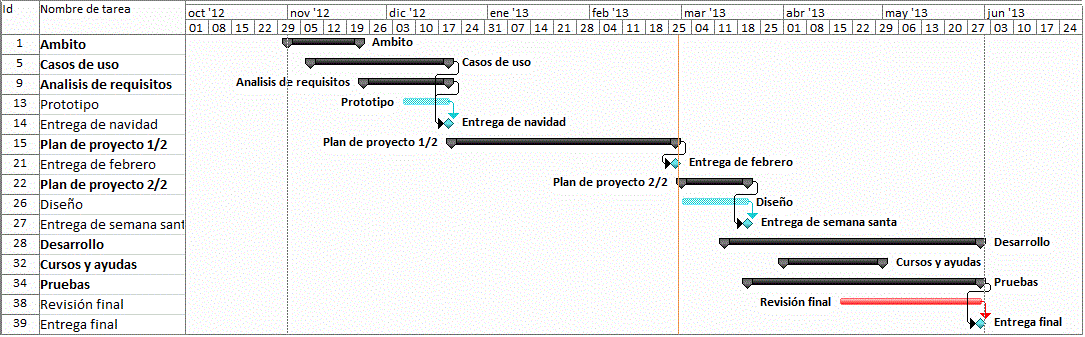
\includegraphics[scale=0.57]{GraficoGantt.png}
	\caption{Diagrama de Gantt}
	\end{figure}

	\section{Gráfico de  Gantt}

	Aquí vemos primero un gráfico de Gant general de todo el proyecto:

	\begin{figure}[!h]
	\centering
	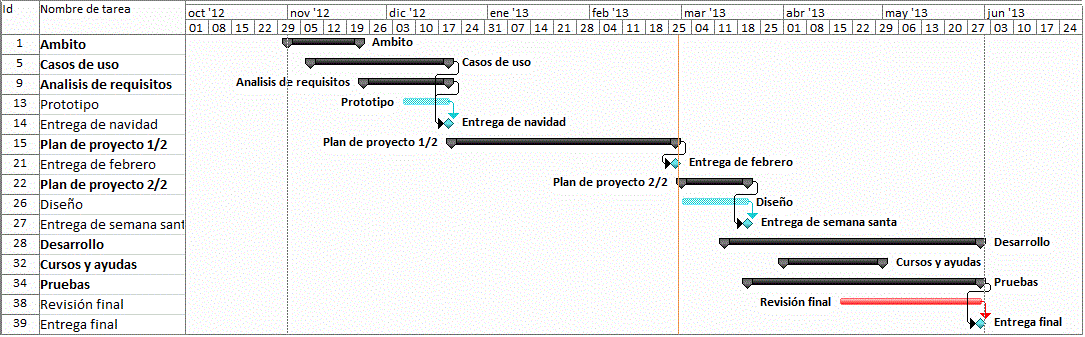
\includegraphics[scale=0.57]{GraficoGantt.png}
	\caption{Diagrama de Gantt}
	\end{figure}

	\newpage

	Aquí tenemos las tareas desglosadas con las fechas:

	\begin{figure}[!h]
	\centering
	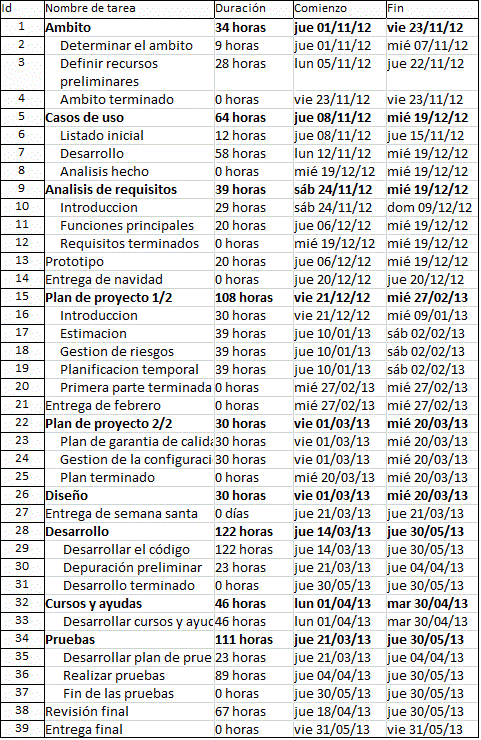
\includegraphics[scale=0.95]{HojaTareas.png}
	\caption{Hoja de las tareas}
	\end{figure}

	\newpage

	Y aquí un gráfico de Gantt desglosado con lo hecho hasta la entrega del proyecto:

	\begin{figure}[!h]
	\centering
	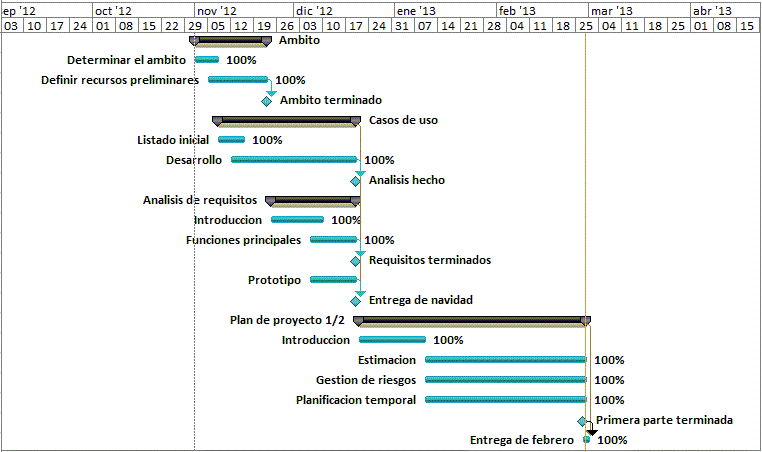
\includegraphics[scale=0.8]{GraficoGanttDetallado.png}
	\caption{Diagrama de Gantt detallado de lo hecho}
	\end{figure}

	\newpage

	\section{Red de tareas}

	Las tareas han estado condicionadas principalmente por las entregas. La entrega de navidad obligó a tener la especificación de requisitos,  los casos de uso y el prototipo preparados.
	 Y la de febrero a tener la primera parte del plan de proyecto terminada. Esta es la red de tareas principal hasta la entrega de febrero:

	\begin{figure}[!h]
	\centering
	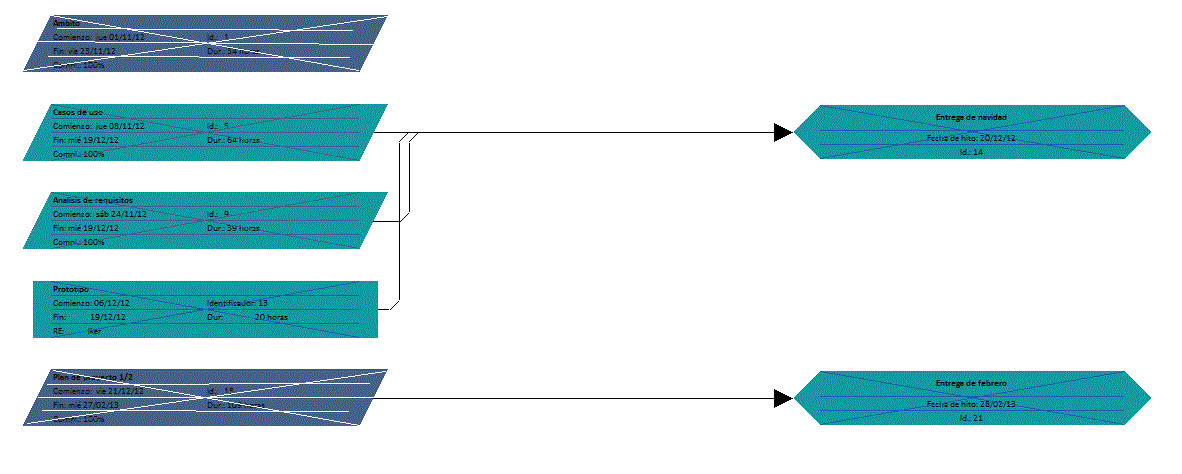
\includegraphics[scale=0.56]{RedTareas.png}
	\caption{Red de tareas}
	\end{figure}

	 Si bien posteriormente la SRS y los casos de uso han sido revisados, puede verse cómo para ser posible la entrega fue necesario tener todo a punto para ese momento.
	Además el prototipo ha sido desechado, y tanto los casos de uso como la SRS están en continua revisión y cambio.

	\newpage

	\section{Tabla de uso de recursos}

	\begin{figure}[!h]
	\centering
	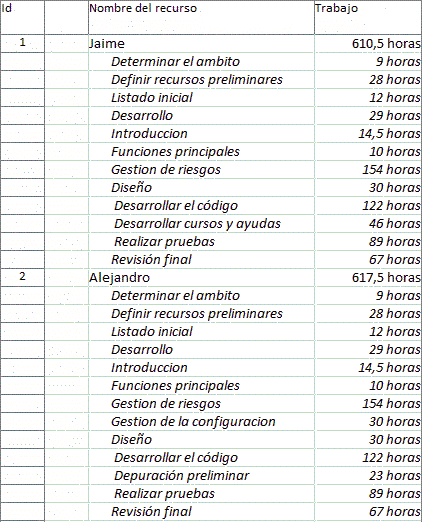
\includegraphics[scale=0.8]{UsoRecursos1.png}
	\caption{Uso de los recursos1}
	\end{figure}

	\begin{figure}[!h]
	\centering
	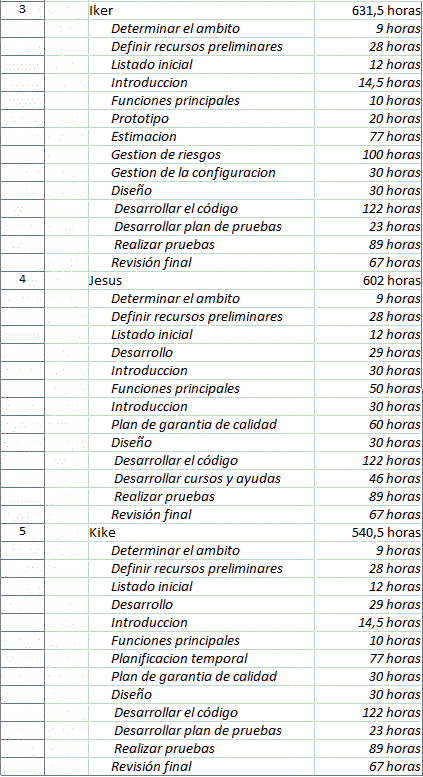
\includegraphics[scale=0.8]{UsoRecursos2.png}
	\caption{Uso de los recursos2}
	\end{figure}

\newpage
\mbox{}
\thispagestyle{empty}						% Hoja en blanco, sin numeros ni nada
\newpage
\setcounter{section}{0}

%JAIME
\chapter{Recursos del proyecto}

	\section{Personal}
		Para el desarrollo del producto se cuenta con un equipo de 5 personas. Este
		equipo se encargará de seguir todos los pasos para conseguir el producto, es
		decir, que se encargarán del total desarrollo del mismo. Esto engloba desde la
		captura de requisitos hasta la puesta en funcionamiento y el mantenimiento del
		producto.\\
		Al ser un equipo pequeño, no hay un reparto bien definido de tareas, ya que todos
		los miembros del equipo participan en todas las actividades. 
		El equipo está formado por: 
		\begin{itemize}
		  \item Jesús Aguirre Pemán (Reichführer)
		  \item Enrique Ballesteros Horcajo
		  \item Jaime Dan Porras Rhee
		  \item Ignacio-Iker Prado Rujas (Führer)
		  \item Alejandro Villarín Prieto
		\end{itemize}
		El Führer es el encargado de organizar y repartir las tareas y el Reichführer suple al Führer en caso de baja.
		Todos los miembros del grupo asesoran al Führer, lo que se puede cumplir fácilmente al ser un grupo reducido.\\
		En los diagramas de Gantt vienen reflejadas las tareas que realizará el equipo y las fechas en las que se realizan.
		
	\section{Hardware y software}

		\subsection{Componentes reutilizables de software}
			Aún no se ha pensado en reutilizar componentes de software ya desarrollados, aunque no se descarta su uso
			en la fase de desarrollo.
		\subsection{Recursos de entorno}
			Para elaborar el producto se requieren numerosas herramientas de hardware y
			software. Estas herramientas son requeridas en todas las fases del proyecto. 
			A continuación se describe cada uno de estos recursos.  \\
			En la fase de captura de requisitos se usaron diversos programas. Los documentos
			se crearon usando \LaTeX , en concreto se usó el programa \texttt{TeXWorks} para editar los documentos.
			También se usó el entorno de programación Eclipse, utlizando el plug-in para \LaTeX\  \texttt{TeXlipse}. 
			Para la realización de presentaciones se ha utilizado el programa \texttt{Microsoft Power Point}.\\
			Para el diseño de Diagramas de casos de uso, se utilizó el programa \texttt{ArgoUML}.\\
			En la fase de planificación y estimación se han utilizado nuevos programas. Para la edición de documentos
			\LaTeX se utilizaron los programas mencionados anteriormente. Para la planificación se ha utilizado el programa
			\texttt{Microsoft Project}, y para la estimación se ha utilizado el programa \texttt{COCOMO-II}.\\ 
			El software se desarrollará sobre el entorno de
			programación Eclipse, utlizando el lenguaje de programación Java. También se
			usarán otros programas informáticos para diseñar los elementos de la interfaz de
			usuario. En cuanto al Hardware, el programa está pensado para que funcione sobre dispositivos como
			tablets o smartphones, tanto los de la plataforma Android como los de la
			plataforma Apple. Por lo tanto, para que el programa pueda ser probado y
			testeado, se necesitarán estos dispositivos. Y para utilizar los programas mencionados anteriormente
			se necesitarán ordenadores personales sobre los que puedan funcionar estos programas.
			No se requerirán herramientas de
			hardware adicionales.


	\section{Lista de recursos}
		\subsection*{Recursos de personal}
			Son los encargados de hacer el producto, desde las primeras fases hasta el desarrollo y mantenimiento.\\
			\begin{itemize}
			  \item Jesús Aguirre Pemán (Reichführer)
			  \item Enrique Ballesteros Horcajo
			  \item Jaime Dan Porras Rhee
			  \item Ignacio-Iker Prado Rujas (Führer)
			  \item Alejandro Villarín Prieto
			\end{itemize}\ \\
			El equipo estará disponible en todo momento.
		\subsection*{Recursos de entorno}
			\begin{itemize}
				  \item \textbf{TeXWorks y TeXlipse}
				  	\begin{itemize}
				  	  \item \textbf{Descripción del recurso: } Programa utlizado para editar los documentos \LaTeX.
				  	  \item \textbf{Informe de disponibilidad: }El programa es de licencia gratuita y estará disponible en 
				  	  			todo momento.
				  	  \item \textbf{Fecha cronológica en la que se requiere el recurso: }El programa será requerido en todo 
				  	  				momento para generar la documentación.
				  	  \item \textbf{Tiempo durante el que será aplicado el recurso: }En todo momento. 
					\end{itemize}
				\item \textbf{ArgoUML}
				  	\begin{itemize}
				  	  \item \textbf{Descripción del recurso: } Programa utilizado para diseñar los diagramas de casos de uso.
				  	  \item \textbf{Informe de disponibilidad: }El programa es de licencia gratuita y estará disponible en 
				  	  			todo momento.
				  	  \item \textbf{Fecha cronológica en la que se requiere el recurso: }El programa será requerido al
				  	  			principio para poner los diagramas en el documento de casos de uso.
				  	  \item \textbf{Tiempo durante el que será aplicado el recurso: }Desde el comienzo hasta la primera entrega. 
					\end{itemize}
				\item \textbf{Microsoft Power Point}
				  	\begin{itemize}
				  	  \item \textbf{Descripción del recurso: } Programa utilizado para realizar presentaciones.
				  	  \item \textbf{Informe de disponibilidad: }El programa está disponible en los laboratorios de la Facultad de Informática.
				  	  \item \textbf{Fecha cronológica en la que se requiere el recurso: }El programa será requerido en cada entrega, para realizar la presentación.
				  	  \item \textbf{Tiempo durante el que será aplicado el recurso: }Desde la primera entrega hasta la última. 
					\end{itemize}
				\item \textbf{Microsoft Project}
				  	\begin{itemize}
				  	  \item \textbf{Descripción del recurso: } Programa utilizado para hacer la planificación del proyecto.
				  	  \item \textbf{Informe de disponibilidad: }El programa está disponible en los laboratorios de la Facultad de Informática.
				  	  \item \textbf{Fecha cronológica en la que se requiere el recurso: }El programa será requerido para hacer la planificación, es decir, en la
				  	  					segunda entrega.
				  	  \item \textbf{Tiempo durante el que será aplicado el recurso: }Desde la primera entrega hasta la segunda. 
					\end{itemize}
				\item \textbf{CoCoMo II}
				  	\begin{itemize}
				  	  \item \textbf{Descripción del recurso: } Programa utilizado para hacer la estimación del proyecto.
				  	  \item \textbf{Informe de disponibilidad: }Disponible a través de Softonic. La licencia se consiguió a través de la UCM.
				  	  \item \textbf{Fecha cronológica en la que se requiere el recurso: }El programa será requerido en la segunda entrega, para
				  	  						realizar la estimación.
				  	  \item \textbf{Tiempo durante el que será aplicado el recurso: }Desde la primera entrega hasta la segunda. 
					\end{itemize}
			\end{itemize} 

\newpage
\mbox{}
\thispagestyle{empty}						% Hoja en blanco, sin numeros ni nada
\newpage
\setcounter{section}{0}



%KIKE & JESUS
%ESTO PARA LA PROXIMA ENTREGA PERO NO SE QUITA, SE QUEDA
%HABRIA QUE DECIRLO AUNQUE SEA
\chapter{Mecanismos de seguimiento y control} La garantía de calidad y el control de cambios serán profundamente analizados en la próxima entrega de documentación.

	\section{Garantía de calidad y control} 
En este apartado comentaremos las revisiones técnicas sobre el producto KIKE HOSTELERIA. Las revisiones formales comenzarán con la fase de codificación.

	\section{Gestión y control de cambios}
Aquí identificaremos, controlaremos y garantizaremos la corrección de la implementación de los cambios, informando de ellos al personal que lo necesite.
El control de versiones nos permitirá identificar y gestionar los diversos documentos y versiones del sistema que tengamos


\newpage
\mbox{}
\thispagestyle{empty}						% Hoja en blanco, sin numeros ni nada
\newpage
%\setcounter{section}{0}
%\part{Apéndices}


\newpage
\mbox{}
\thispagestyle{empty}						% Hoja en blanco, sin numeros ni nada, al final del documento
\newpage

\end{document}

%ESQUEMA DEL PLAN DE PROYECTO SEGUN PRESSMAN: SI TENÉIS DUDAS VIENE BASTANTE EXPLICADO EN EL LIBRO DE PRESSMAN
%LA DISTRIBUCION NO ES DEFINITIVA, EN FUNCION DE LO LARGA QUE SEA CADA PARTE LOS QUE ACABEN ANTES AYUDAN AL RESTO

%JESUS
1. Introducción
	1.1 Propósito del plan
	1.2 Ámbito del proyecto y objetivos
		1.2.1 Declaración del ámbito
		1.2.2 Funciones principales
		1.2.3 Aspectos de rendimiento
		1.2.4 Restricciones y técnicas de gestión
	1.3 Modelo de proceso

%IKER
2. Estimaciones del proyecto
	2.1 Datos históricos
	2.2 Técnicas de estimación
	2.3 Estimaciones de esfuerzo, coste y duración

%VILLARIN & JAIME
3. Estrategia de gestión del riesgo 
	3.1 Análisis del riesgo
	3.2 Estudio de los riesgos
	3.3 Plan de gestión del riesgo

%KIKE
4. Planificación temporal
	4.1 Estructura de descomposición del trabajo/Planificación temporal
	4.2 Gráfico de  Gantt
	4.3 Red de tareas
	4.4 Tabla de uso de recursos

%JAIME
5. Recursos del proyecto 
	5.1 Personal
	5.2 Hardware y software
	5.3 Lista de recursos

%JESUS
6. Organización del personal
	6.1 Estructura de equipo (si procede)
	6.2 Informes de gestión
%KIKE & JESUS
7. Mecanismos de seguimiento y control


	7.1 Garantía de calidad y control
	7.2 Gestión y control de cambios 

8. Apéndices